\chapter{Context and importance of this research}
\label{ch:context}
This chapter covers the basic context of the research,
regarding the location and past studies of the Yolngu calendar;
finds a gap in the literature and surveys relevant fields;
and lays out the overarching methodology of and strategy for this research.


\section{Context}
This section is at notes/draft stage.

\begin{figure}[h]
    \centering
    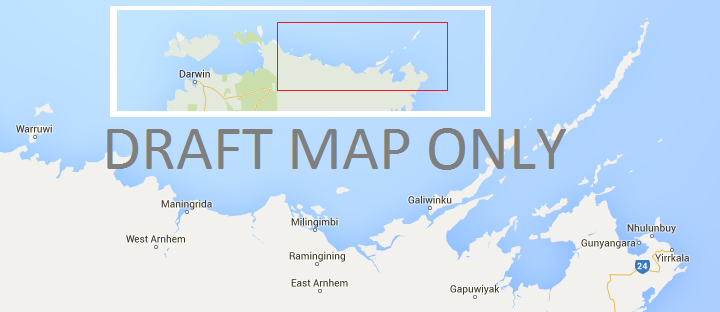
\includegraphics[width=\textwidth]{mapdraft.png}
    \caption[Map showing the study area, NE Arnhem Land]{
        Map showing the study area, NE Arnhem Land.
        Analysis in \autoref{ch:quantify} uses weather observations from several of the towns shown.
        }
    \label{fig:arnhem-map}
\end{figure}


This study focusses on North-East Arnhem Land, particularly Elcho Island
and the town of Galiwinku.  Figure~\ref{fig:arnhem-map} shows the study area.
Qualitative seasonality is described for Galiwinku and Milingimbi;
quantitative weather observations are from Waruwi, Maningrida, Milingimbi,
Galiwinku, and Nhulunbuy.

These sites are all in Yolngu country, in the Anrhem Coast bioregion \citep{ens2014}.
The landscape is dominated by tropical woodland, from mangroves on the coastline 
through dense forest to more open woody grasslands further inland.

Yolngu have a tradition of engagement across cultures, including
the Macassan trade with Indonesia in the 1700s and engagement with Methodist
missionaries throughout the 1900s.

The Yirrkala Bark Petition (\autoref{fig:bark-petition}) marks a crucial
point in the Australian land rights movement, recognised by indigenous and
non-indigenous people alike.  It is also prone to misinterpretation by those
who see a document in two languages with a decorative border: the border
is the most important part!  (see caption, expand this section)


\begin{wrapfigure}{R}{0.5\textwidth}
    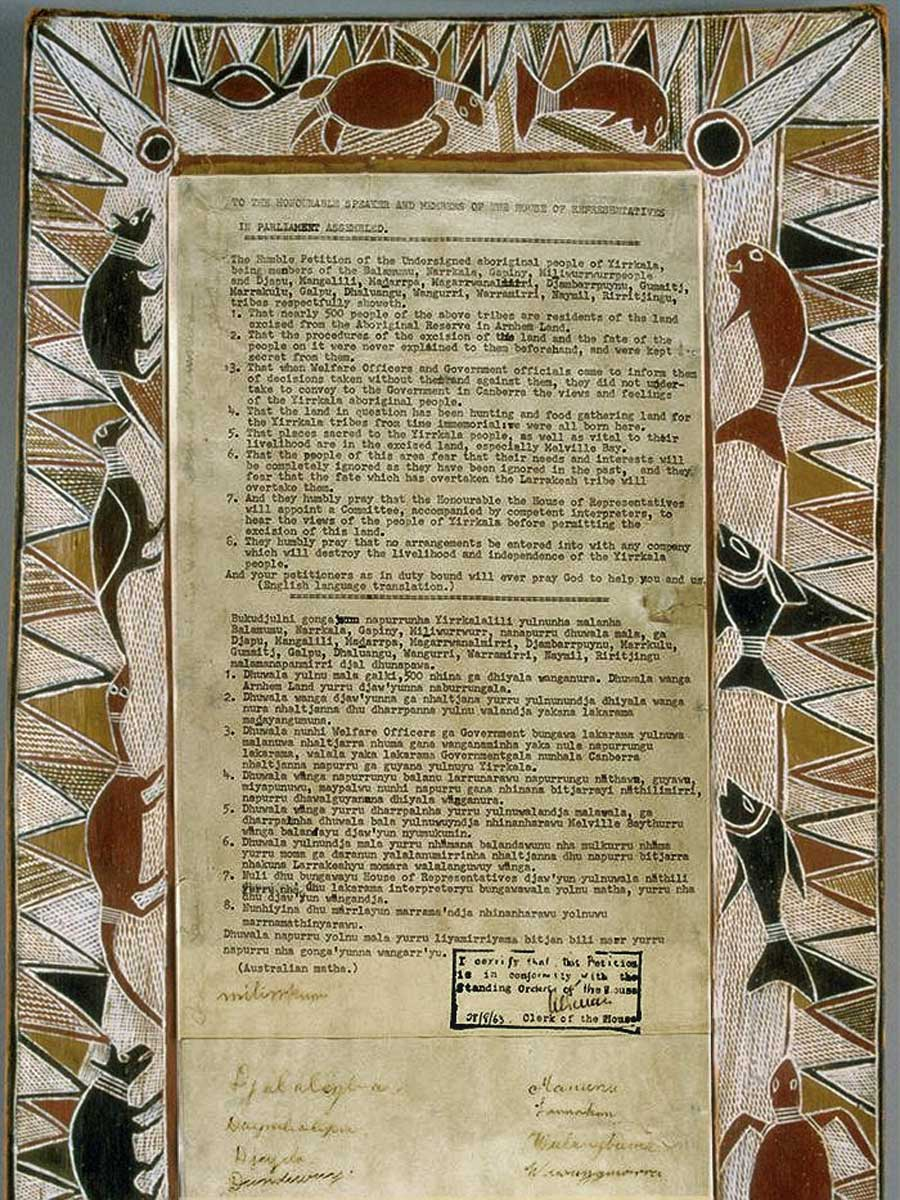
\includegraphics[width=\linewidth]{bark-petition.jpg}
    \caption[The Yirrkala Bark Petition]{
        The Yirrkala Bark Petition, 1963.
        The Bark Petition concerns the bauxite mining lease granted at Nhulunbuy
        without consultation with Yolngu, and helped kick-start the Australian
        land rights movement.

        The petition is presented in three ways: text in English,
        text in Yolngu Matha, and in the border.
        This painting is not a decoration; it is a reproduction of
        the title deeds to the ancestoral estates of the signatories -
        and the most important part of the document.
        }
    \label{fig:bark-petition}
\end{wrapfigure}


In a letter inviting collaboration on this research (see \autoref{sec:ethics}),
a senior Yonlgu man explained that:

\blockquote{
    For Yolngu (the people of North Eastern Arnhem Land) it is the Liyagadhaman
    who carry within them the wisdom and knowledge of these matters.
    It is right that in this research you have approached me to talk about these
    things. I can also introduce you to others who have this knowledge.  ...

    Yolngu have made careful observation of the ways of nature and the seasons
    over the millennia and have passed on that knowledge down the generations.
    We know the changes that are taking place in the seasons and I am willing
    to talk with you about what I have seen happening around me.
}




The BOM describes the 
climate as ``hot and humid'', with daytime temperatures between 25 and 40 
degrees year-round.  Rainfall and humidity are dominated by monsoon 
seasonality, and the seasons are commonly described by non-indigenous residents 
as “the Wet” and “the Dry” – though after a few years many also recognise “the 
Buildup” of pre-wet humidity \citep{willmett2009}.

The key meteorological determinants of seasonality are temperature (especially 
night-time), rainfall, humidity, and wind strength and direction.  The annual 
cycle is driven primarily by the Indian Ocean monsoon.  The seasonal effect of 
temperature is felt most strongly at night, as daytime temperatures are very 
consistent and the latent heat of available water has a strong effect.

However, wet/dry/buildup misses important nuance in the seasonality of the 
area.  \autoref{fig:yolngu-seasons} shows one summary of Yolngu seasonality,
with significantly more seasons.  \citet{woodward2012b} notes
\blockquote{
    four factors that interconnect within each of the seasonal
    knowledge systems; a focus on resource use, knowledge of complex
    ecological indicators to facilitate resource collection,
    knowledge of meteorological phenomena and a strong
    metaphysical/spiritual understanding.
}

